\documentclass[]{article}
\usepackage[utf8]{inputenc}
\usepackage[spanish]{babel}
\usepackage{graphicx, graphics, float, fancyhdr, titling, caption, subcaption, amsmath}
\usepackage{listings,xcolor}
\usepackage[a4paper, total={6in, 9.5in}]{geometry}
\usepackage{fancyhdr}
\usepackage{hyperref}   %para que funcione addcontentsline debe ser la ultima que se cargue

\usepackage{blindtext}
\usepackage{mwe}

%\setcounter{secnumdepth}{-2}       %Poner solo esto si no se quieren numero delante de las secciones y niveles inferiores.

\renewcommand{\footrulewidth}{0.4pt}
\title{

\includegraphics[width=1.75in]{imagenes/UGR-Logo.png} \\
\vspace*{1in}
\textbf{Memoria de la Práctica 6} \\
Animación por Ordenador \\
\vspace*{0.5in}}
\author{Andrés Merlo Trujillo \\
andresmerlo@correo.ugr.es \\
77147239H \\ 
\vspace*{0.5in} \\
E.T.S. de Ingenierías Informática y de Telecomunicación \\
\textbf{Universidad de Granada}} \date{\today}

\hypersetup{
    colorlinks=true,
    linkcolor=black,
    citecolor=black
}

\renewcommand\maketitlehooka{\null\mbox{}\vfill}
\renewcommand\maketitlehookd{\vfill\null}

\definecolor{codegreen}{rgb}{0,0.6,0}
\definecolor{codegray}{rgb}{0.5,0.5,0.5}
\definecolor{codepurple}{rgb}{0.58,0,0.82}
\definecolor{backcolour}{rgb}{0.95,0.95,0.92}

\lstdefinestyle{mystyle}{
    backgroundcolor=\color{backcolour},   
    commentstyle=\color{codegreen},
    keywordstyle=\color{magenta},
    numberstyle=\tiny\color{codegray},
    stringstyle=\color{codepurple},
    basicstyle=\ttfamily\footnotesize,
    breakatwhitespace=false,         
    breaklines=true,                 
    captionpos=b,                    
    keepspaces=true,                 
    numbers=left,                    
    numbersep=5pt,                  
    showspaces=false,                
    showstringspaces=false,
    showtabs=false,                  
    tabsize=2,
    literate=
  {á}{{\'a}}1 {é}{{\'e}}1 {í}{{\'i}}1 {ó}{{\'o}}1 {ú}{{\'u}}1
  {Á}{{\'A}}1 {É}{{\'E}}1 {Í}{{\'I}}1 {Ó}{{\'O}}1 {Ú}{{\'U}}1
  {à}{{\`a}}1 {è}{{\`e}}1 {ì}{{\`i}}1 {ò}{{\`o}}1 {ù}{{\`u}}1
  {À}{{\`A}}1 {È}{{\`E}}1 {Ì}{{\`I}}1 {Ò}{{\`O}}1 {Ù}{{\`U}}1
  {ä}{{\"a}}1 {ë}{{\"e}}1 {ï}{{\"i}}1 {ö}{{\"o}}1 {ü}{{\"u}}1
  {Ä}{{\"A}}1 {Ë}{{\"E}}1 {Ï}{{\"I}}1 {Ö}{{\"O}}1 {Ü}{{\"U}}1
  {â}{{\^a}}1 {ê}{{\^e}}1 {î}{{\^i}}1 {ô}{{\^o}}1 {û}{{\^u}}1
  {Â}{{\^A}}1 {Ê}{{\^E}}1 {Î}{{\^I}}1 {Ô}{{\^O}}1 {Û}{{\^U}}1
  {ã}{{\~a}}1 {ẽ}{{\~e}}1 {ĩ}{{\~i}}1 {õ}{{\~o}}1 {ũ}{{\~u}}1
  {Ã}{{\~A}}1 {Ẽ}{{\~E}}1 {Ĩ}{{\~I}}1 {Õ}{{\~O}}1 {Ũ}{{\~U}}1
  {œ}{{\oe}}1 {Œ}{{\OE}}1 {æ}{{\ae}}1 {Æ}{{\AE}}1 {ß}{{\ss}}1
  {ű}{{\H{u}}}1 {Ű}{{\H{U}}}1 {ő}{{\H{o}}}1 {Ő}{{\H{O}}}1
  {ç}{{\c c}}1 {Ç}{{\c C}}1 {ø}{{\o}}1 {Ø}{{\O}}1 {å}{{\r a}}1 {Å}{{\r A}}1
  {€}{{\euro}}1 {£}{{\pounds}}1 {«}{{\guillemotleft}}1
  {»}{{\guillemotright}}1 {ñ}{{\~n}}1 {Ñ}{{\~N}}1 {¿}{{?`}}1 {¡}{{!`}}1,
  extendedchars=true
}

\lstset{style=mystyle}

\lstdefinelanguage{MaxScript}{
  keywords={break, case, catch, collect, continue, coordsys, default, do, else, exit, false, for, fn, global, if, in, local, macroScript, not, of, on, plugin, return, rollouts, silent, struct, then, to, true, try, undo, utilities, when, while, quat, rotate, move, normalize, distance, ray, intersectRay},
  keywordstyle=\color{blue}\bfseries,
%   ndkeywords={!=, #, #_, ##, %, &amp;, \&, \&, *, **, +, -, /, //, :, &lt;&lt;, &gt;&gt;, &lt;=, &gt;=, ==, ^, ~, ~=, +=, -=, *=, /=, //=, ^=, &=, &lt;&lt;=, &gt;&gt;=},
%   ndkeywordstyle=\color{red}\bfseries,
  identifierstyle=\color{black},
  sensitive=true,
  comment=[l]{--},
  morecomment=[s]{/*}{*/},
  commentstyle=\color{codegreen}\ttfamily,
  stringstyle=\color{purple}\ttfamily,
  morestring=[b]',
  morestring=[b]"
}

\begin{document}
\begin{titlingpage}
\maketitle
\end{titlingpage}

\tableofcontents

\newpage

\pagestyle{fancy}   %a partir de comienza el header (se salta el indice y portada)
\fancyhead[L]{Andrés Merlo Trujillo}
\fancyhead[R]{Animación por Ordenador}
%\section{Ejercicio 1}
%\begin{figure}[H]
%    \centering
%    \includegraphics[width=\textwidth]{imagenes/passwdfile.png}
%\end{figure}


\section{Introducción}

En esta práctica se pide crear un modelo sencillo y construir un \textit{rig} que permita controlar la animación.

\bigskip

En mi caso, he decidido crear una excavadora que puede girar sobre su propio eje.

\begin{figure}[H]
   \centering
   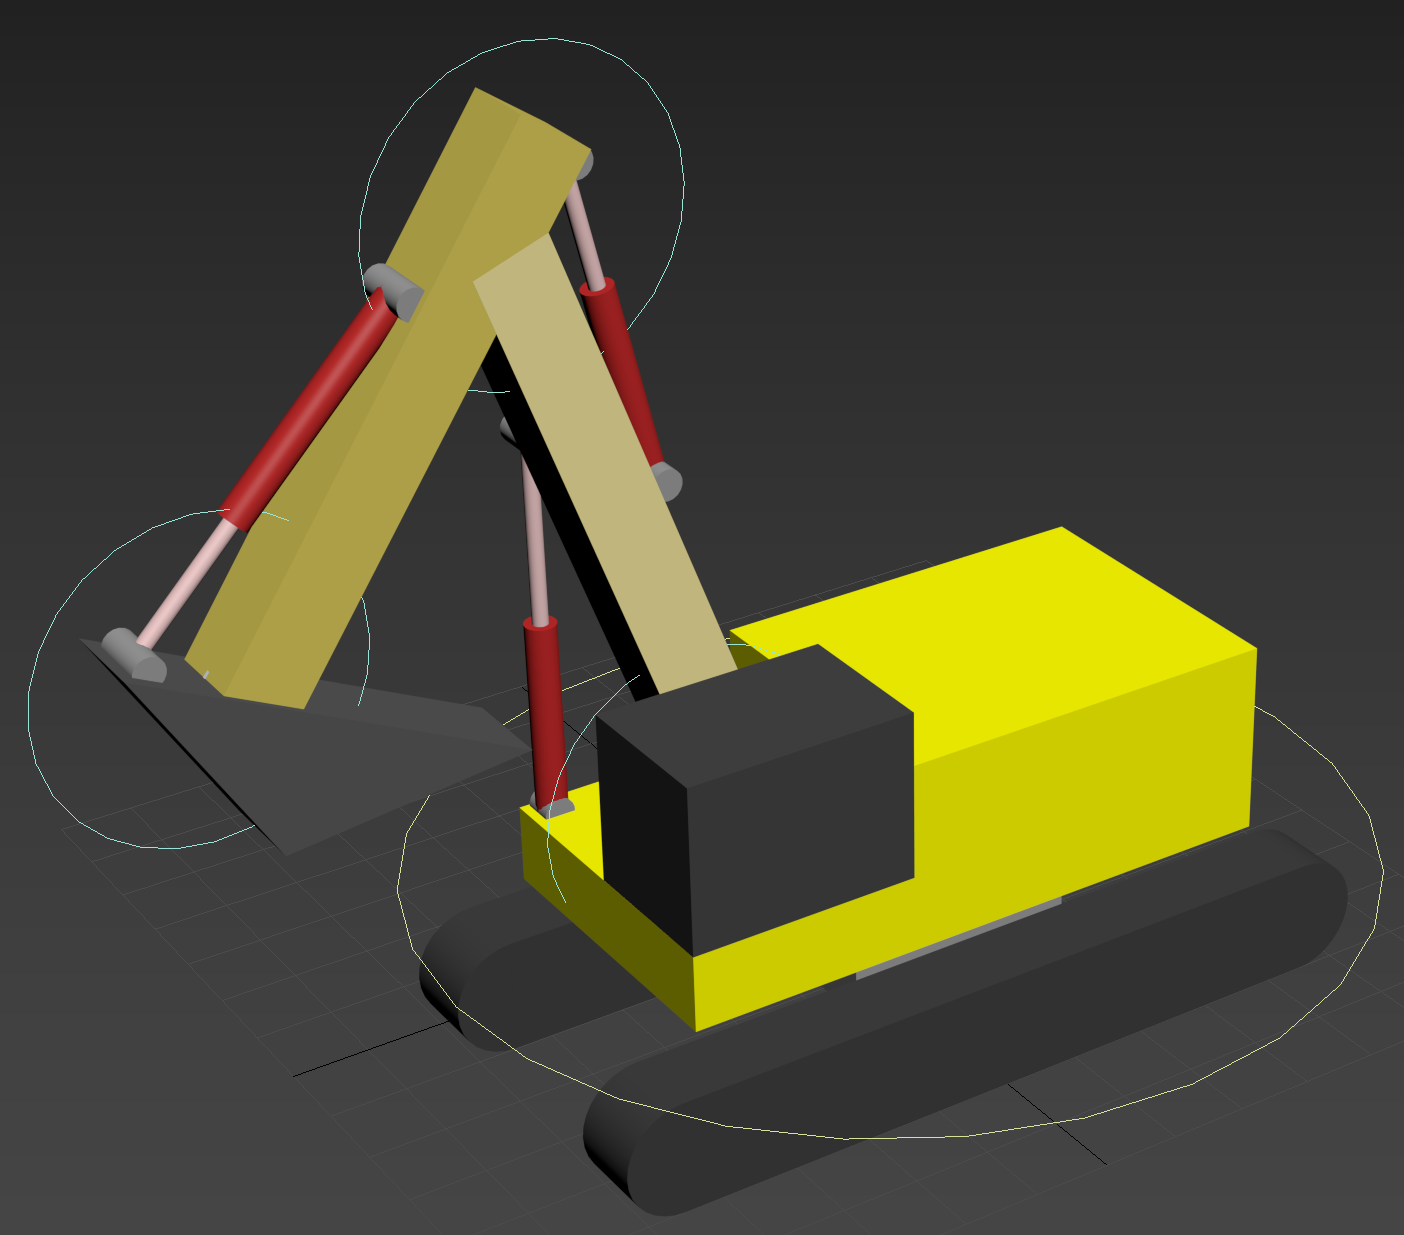
\includegraphics[width=0.5\textwidth]{imagenes/excavadora.png}
   \caption{Modelo final de la excavadora.}
\end{figure}

En las siguientes secciones explicaré el proceso de creación del modelo:
\section{Posición}

Para realizar el movimiento de la pelota, es necesario utilizar el vector Up de la pelota guía y multiplicarlo por -1, de forma que el vector resultante mire hacia abajo. Una vez realizado esto, se debe lanzar un rayo para intersecar la superficie, así se obtiene un vector con la posición en la que ha intersecado.

\bigskip

Finalmente, se modifica el valor \textit{pos} de la pelota para que sea igual que el punto de colisión del suelo. Al realizar esto, la pelota aparecerá hundida en el suelo, por lo que es necesario levantarla. Para ello, se debe utilizar el vector normal de la superficie del suelo con la que ha intersecado el rayo y multiplicarlo por el radio de la pelota, para que tenga dicho valor de módulo. Con este vector obtenido, solo es necesario ejecutar el comando \verb|move| en la pelota una vez para sacarla del suelo.

% foto de hundido y despues.
\begin{figure}[H]
    \centering 
	\begin{subfigure}[t]{0.3\textwidth}
	    \centering
	    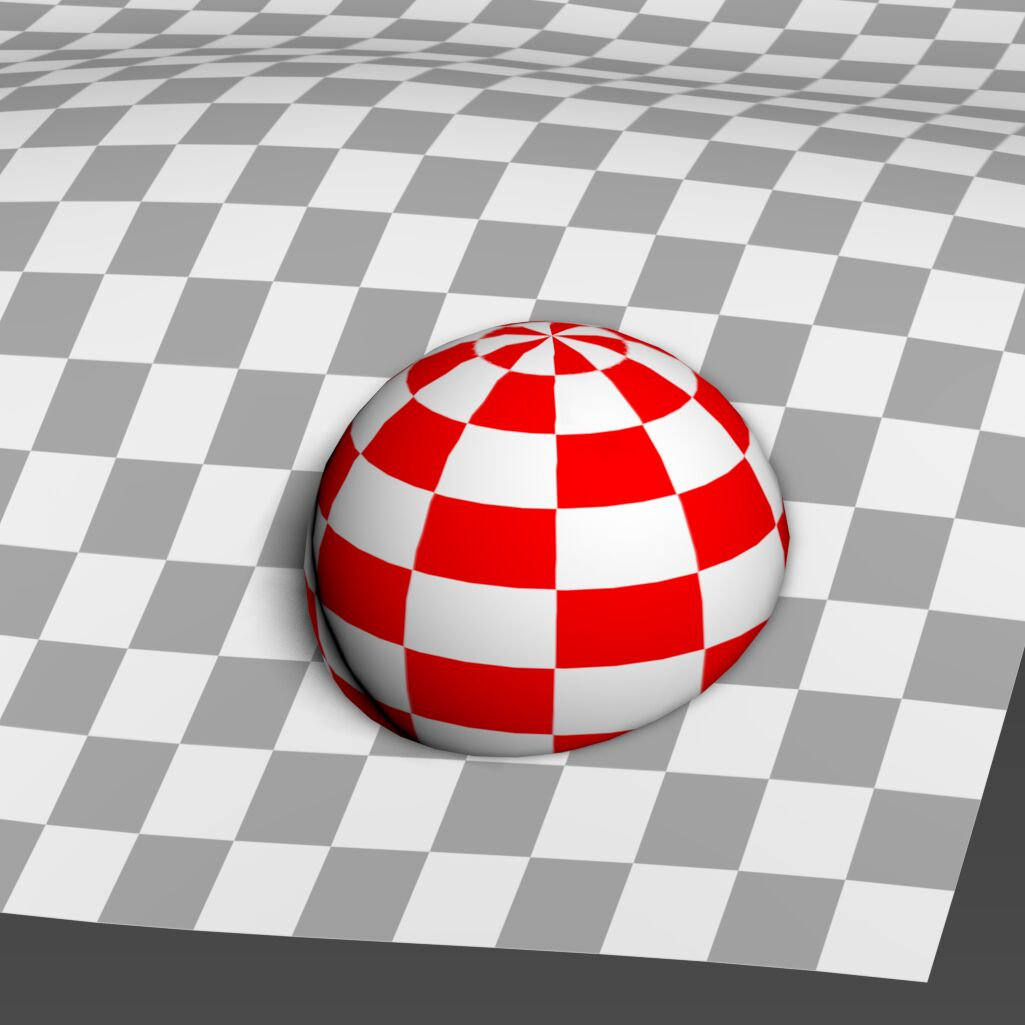
\includegraphics[width=\textwidth]{imagenes/posicion/hundido.jpg}
        \caption{Pelotas hundida en el suelo.}
    \end{subfigure}
    \hspace{20px}
	\begin{subfigure}[t]{0.3\textwidth}
	    \centering
	    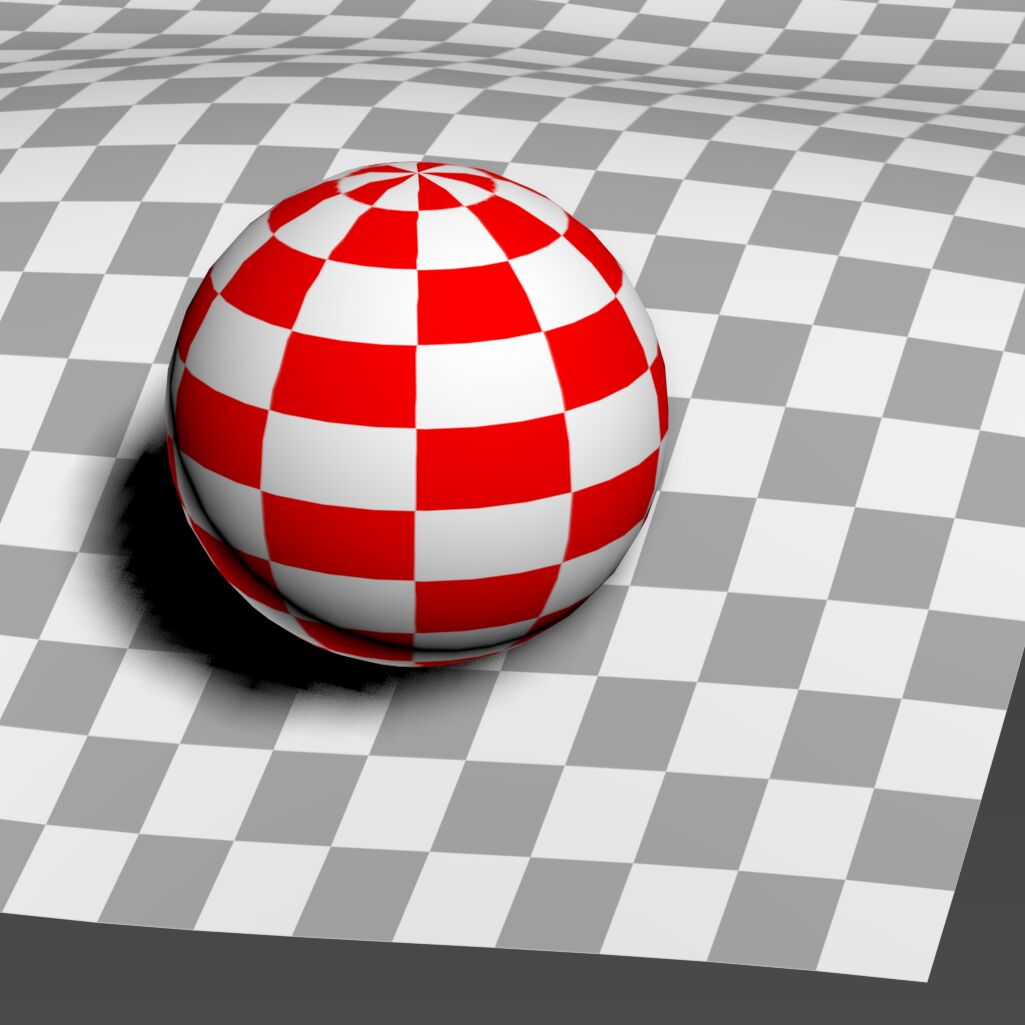
\includegraphics[width=\textwidth]{imagenes/posicion/normal.jpg}
        \caption{Pelotas correctamente posicionada.}
    \end{subfigure}    
    \caption{Diferencia entre usar el comando \texttt{move} y no usarlo.}
\end{figure}

La función para implementar esta funcionalidad es el siguiente:

% codigo
\lstinputlisting[language=MaxScript,firstline=21,lastline=37 ]{../eje_MerloTrujilloAndres_AO_P6.ms}

\bigskip
\newpage

Y a continuación hay capturas con la pelota en distintos lugares y posicionada correctamente, pero sin rotar, que se hará en la siguiente sección:

% dos o tres fotos de la pelota a distintas alturas.

\begin{figure}[H]
    \centering 
	\begin{subfigure}[t]{0.48\textwidth}
	    \centering
	    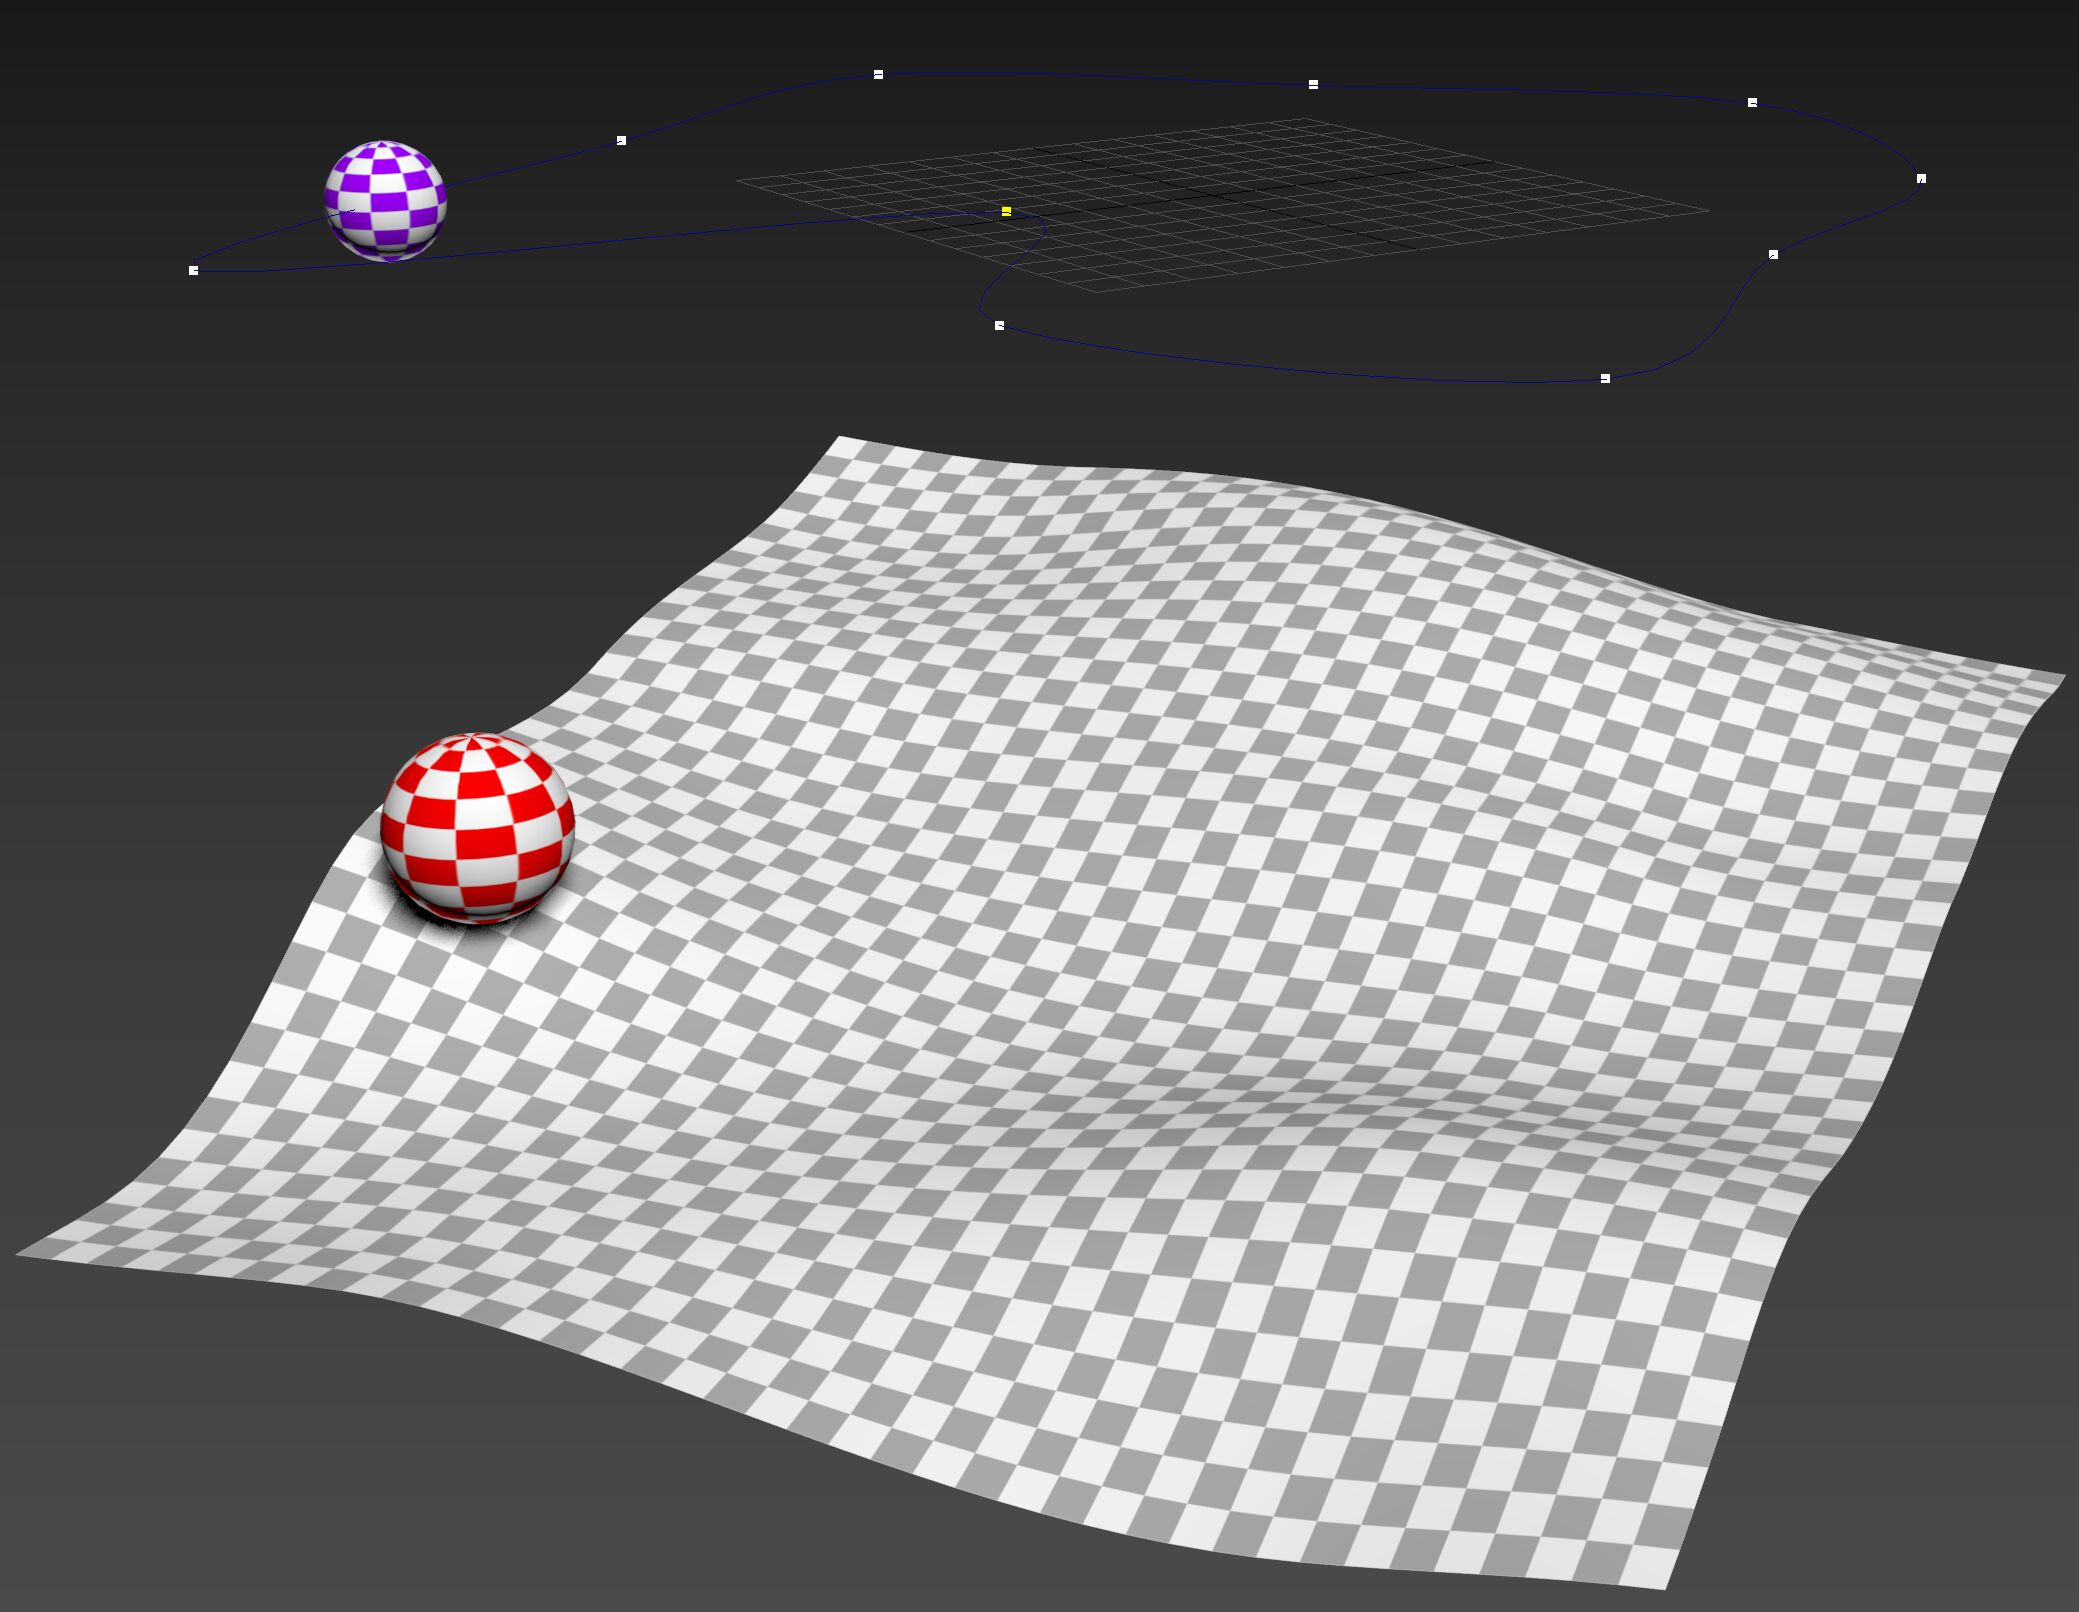
\includegraphics[width=\textwidth]{imagenes/posicion/100.jpg}
        \caption{Pelotas en el instante 100.}
    \end{subfigure}
    \hfill 
    %\par\bigskip %si se desea dejar un margen entre la imagen de arriba y de abajo. SOLO SE PUEDE USAR HFILL O ESTE
	\begin{subfigure}[t]{0.48\textwidth}
	    \centering
	    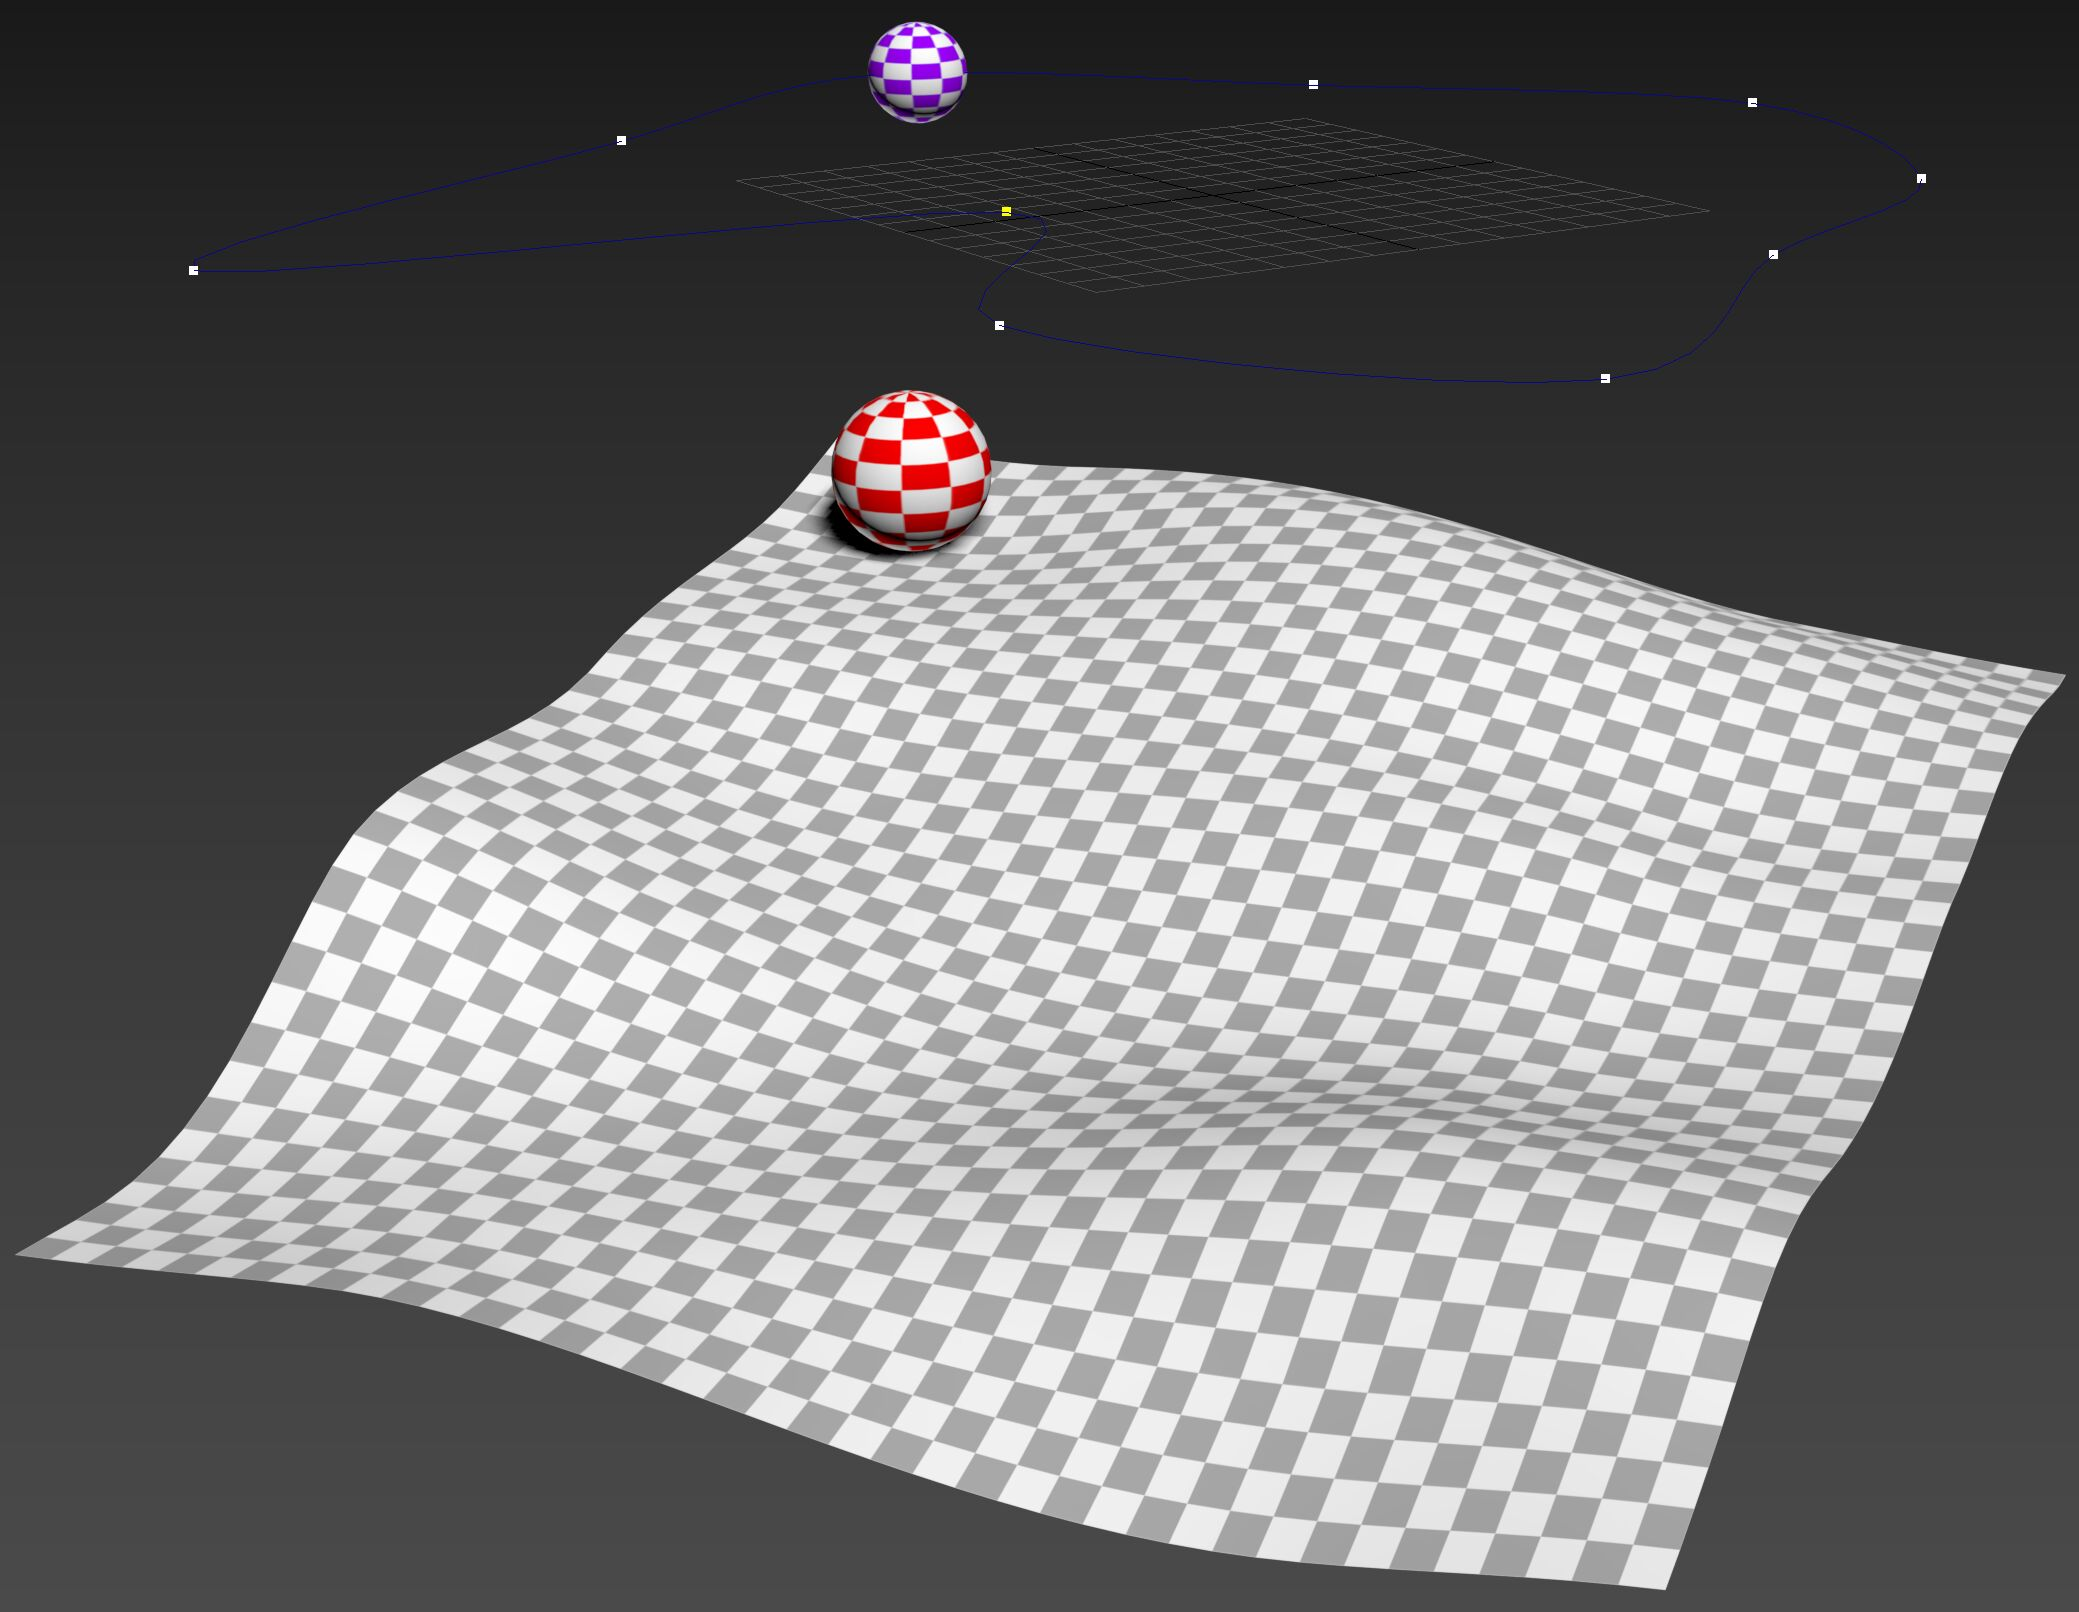
\includegraphics[width=\textwidth]{imagenes/posicion/185.jpg}
        \caption{Pelotas en el instante 185.}
    \end{subfigure}    
    \par\bigskip
	\begin{subfigure}[t]{0.48\textwidth}
	    \centering
	    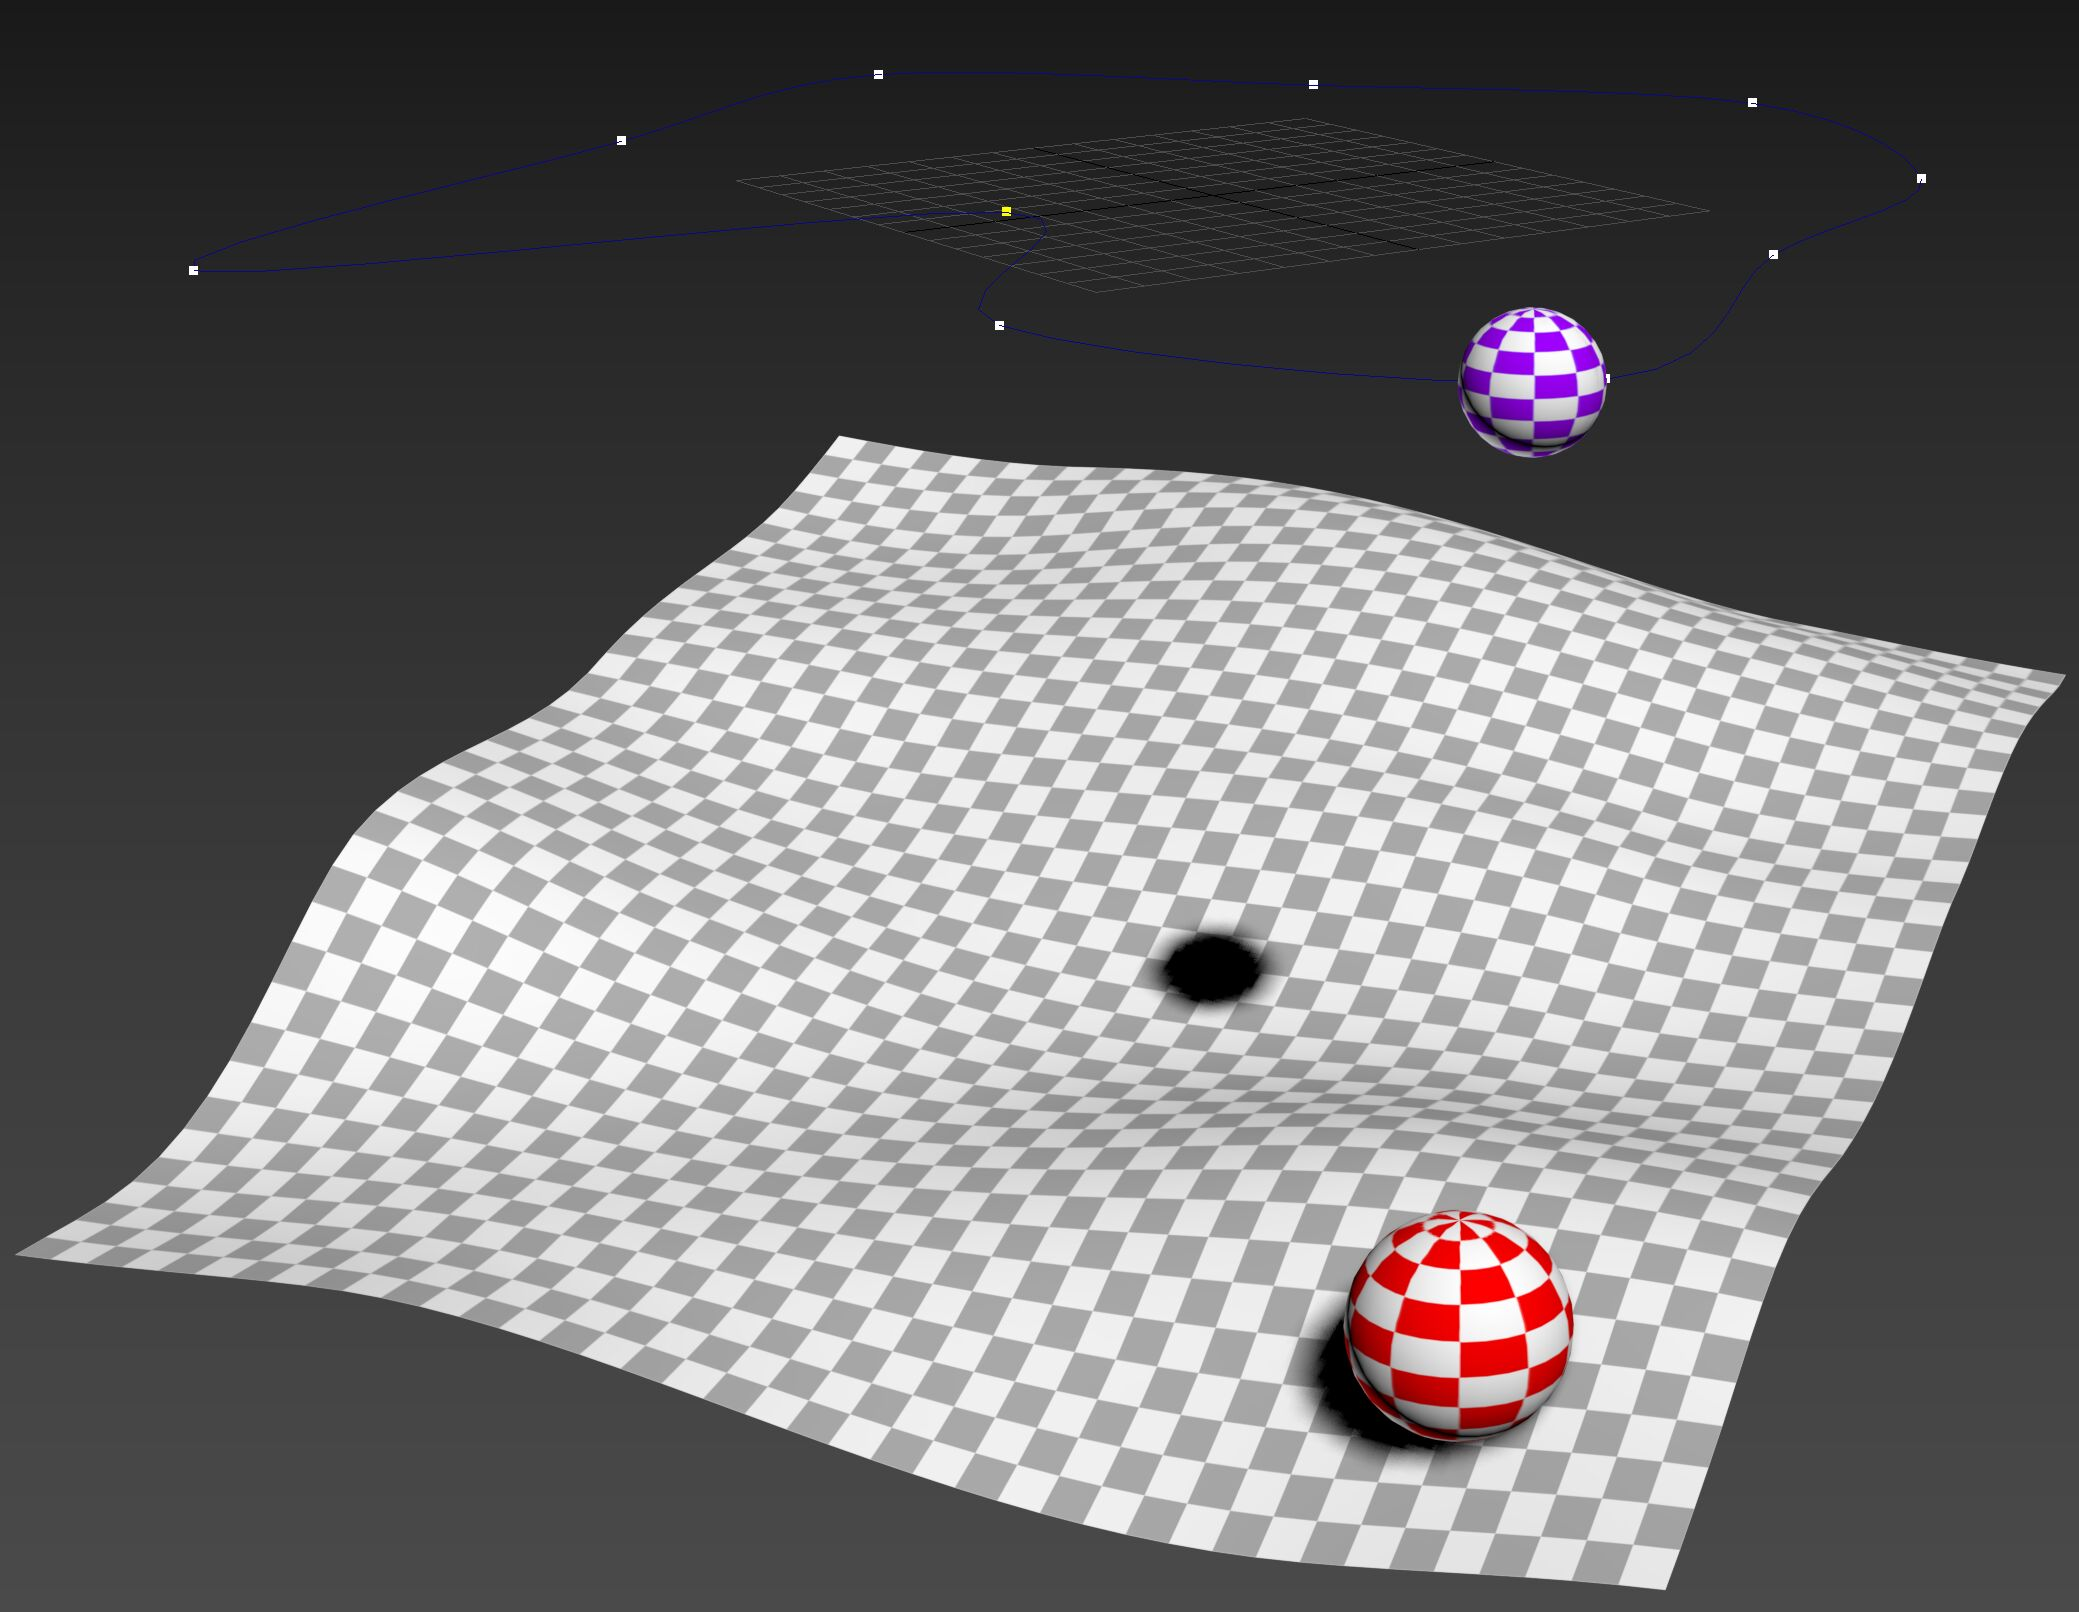
\includegraphics[width=\textwidth]{imagenes/posicion/410.jpg}
        \caption{Pelotas en el instante 410.}
    \end{subfigure}        
    \caption{Visualización de algunos instantes de la animación sin usar la rotación.}
\end{figure}
\newpage

\section{Rotación}

Para realizar la rotación, es necesario saber la posición en el instante anterior de la pelota, y la posición en el instante actual, para así obtener el vector con la dirección (por simplicidad lo llamaré ``v''). También es necesario obtener ``v'' normalizado para realizar otros cálculos (lo llamaré ``w'').

\bigskip

Una vez obtenido ``w'' y haciendo uso del vector normal de la superficie obtenido en la intersección de rayos, se hace el producto vectorial para así obtener el eje de giro.

\bigskip

Por último, para saber cuantos grados debe rotar la pelota, es necesario calcular la distancia de ``v'', de forma que así se obtenga la distancia que ha recorrido. Después, se debe utilizar la fórmula de la longitud del arco de circunferencia, poniendo como incógnita el ángulo. Se debe hacer así porque hay que convertir la distancia recta en distancia circular, para calcular los ángulos. 

\bigskip

La fórmula de la longitud de la circunferencia, cuya incógnita es el ángulo, es: $\alpha = \frac{180 \cdot L}{\pi \cdot r} $, donde L es la longitud recorrida y r el radio de la pelota.

\bigskip

El código para realizar esto es:

% codigo [firstline=300,lastline=500]
\lstinputlisting[language=MaxScript,firstline=40,lastline=65]{../eje_MerloTrujilloAndres_AO_P6.ms}

Cabe destacar que esta función no se debe ejecutar en el primer instante, al necesitar tener el valor de posición de la pelota guía en el instante anterior, por lo que hay que esperar al segundo instante para que empiece a funcionar.

\bigskip
\newpage

A continuación muestro algunas imágenes de la rotación:

% dos o tres fotos en los mismos instantes que antes de la traslacion
\begin{figure}[H]
    \centering 
	\begin{subfigure}[t]{0.48\textwidth}
	    \centering
	    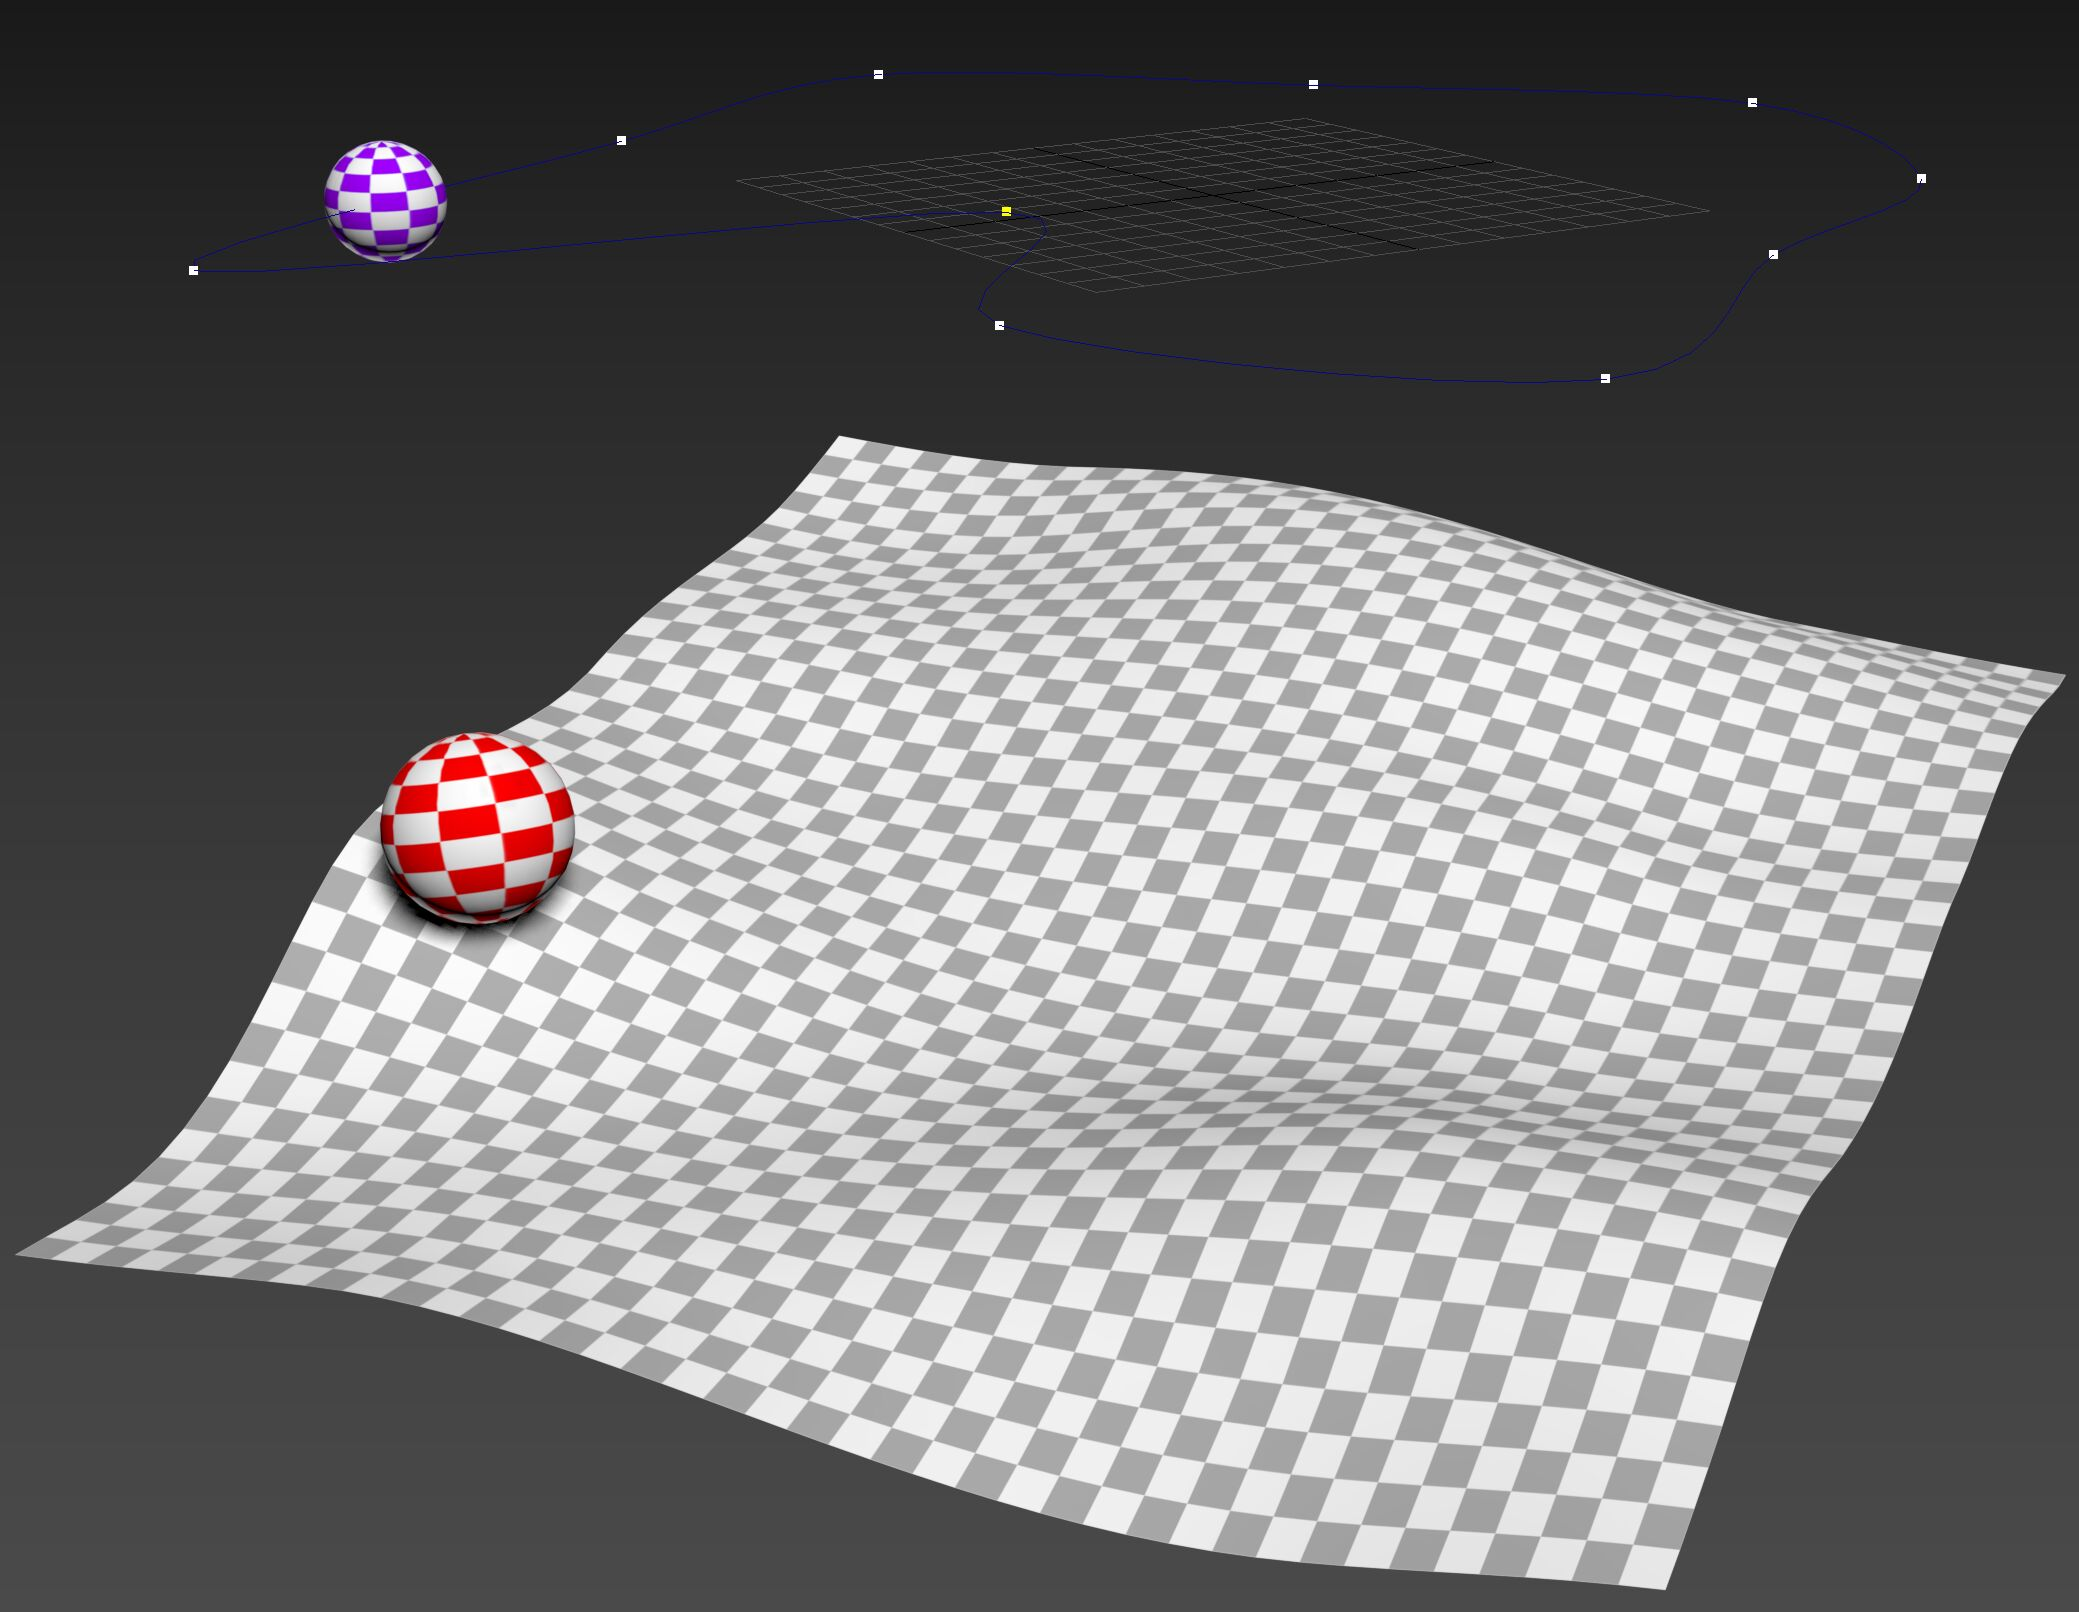
\includegraphics[width=\textwidth]{imagenes/rotacion/100.jpg}
        \caption{Pelotas en el instante 100.}
    \end{subfigure}
    \hfill 
	\begin{subfigure}[t]{0.48\textwidth}
	    \centering
	    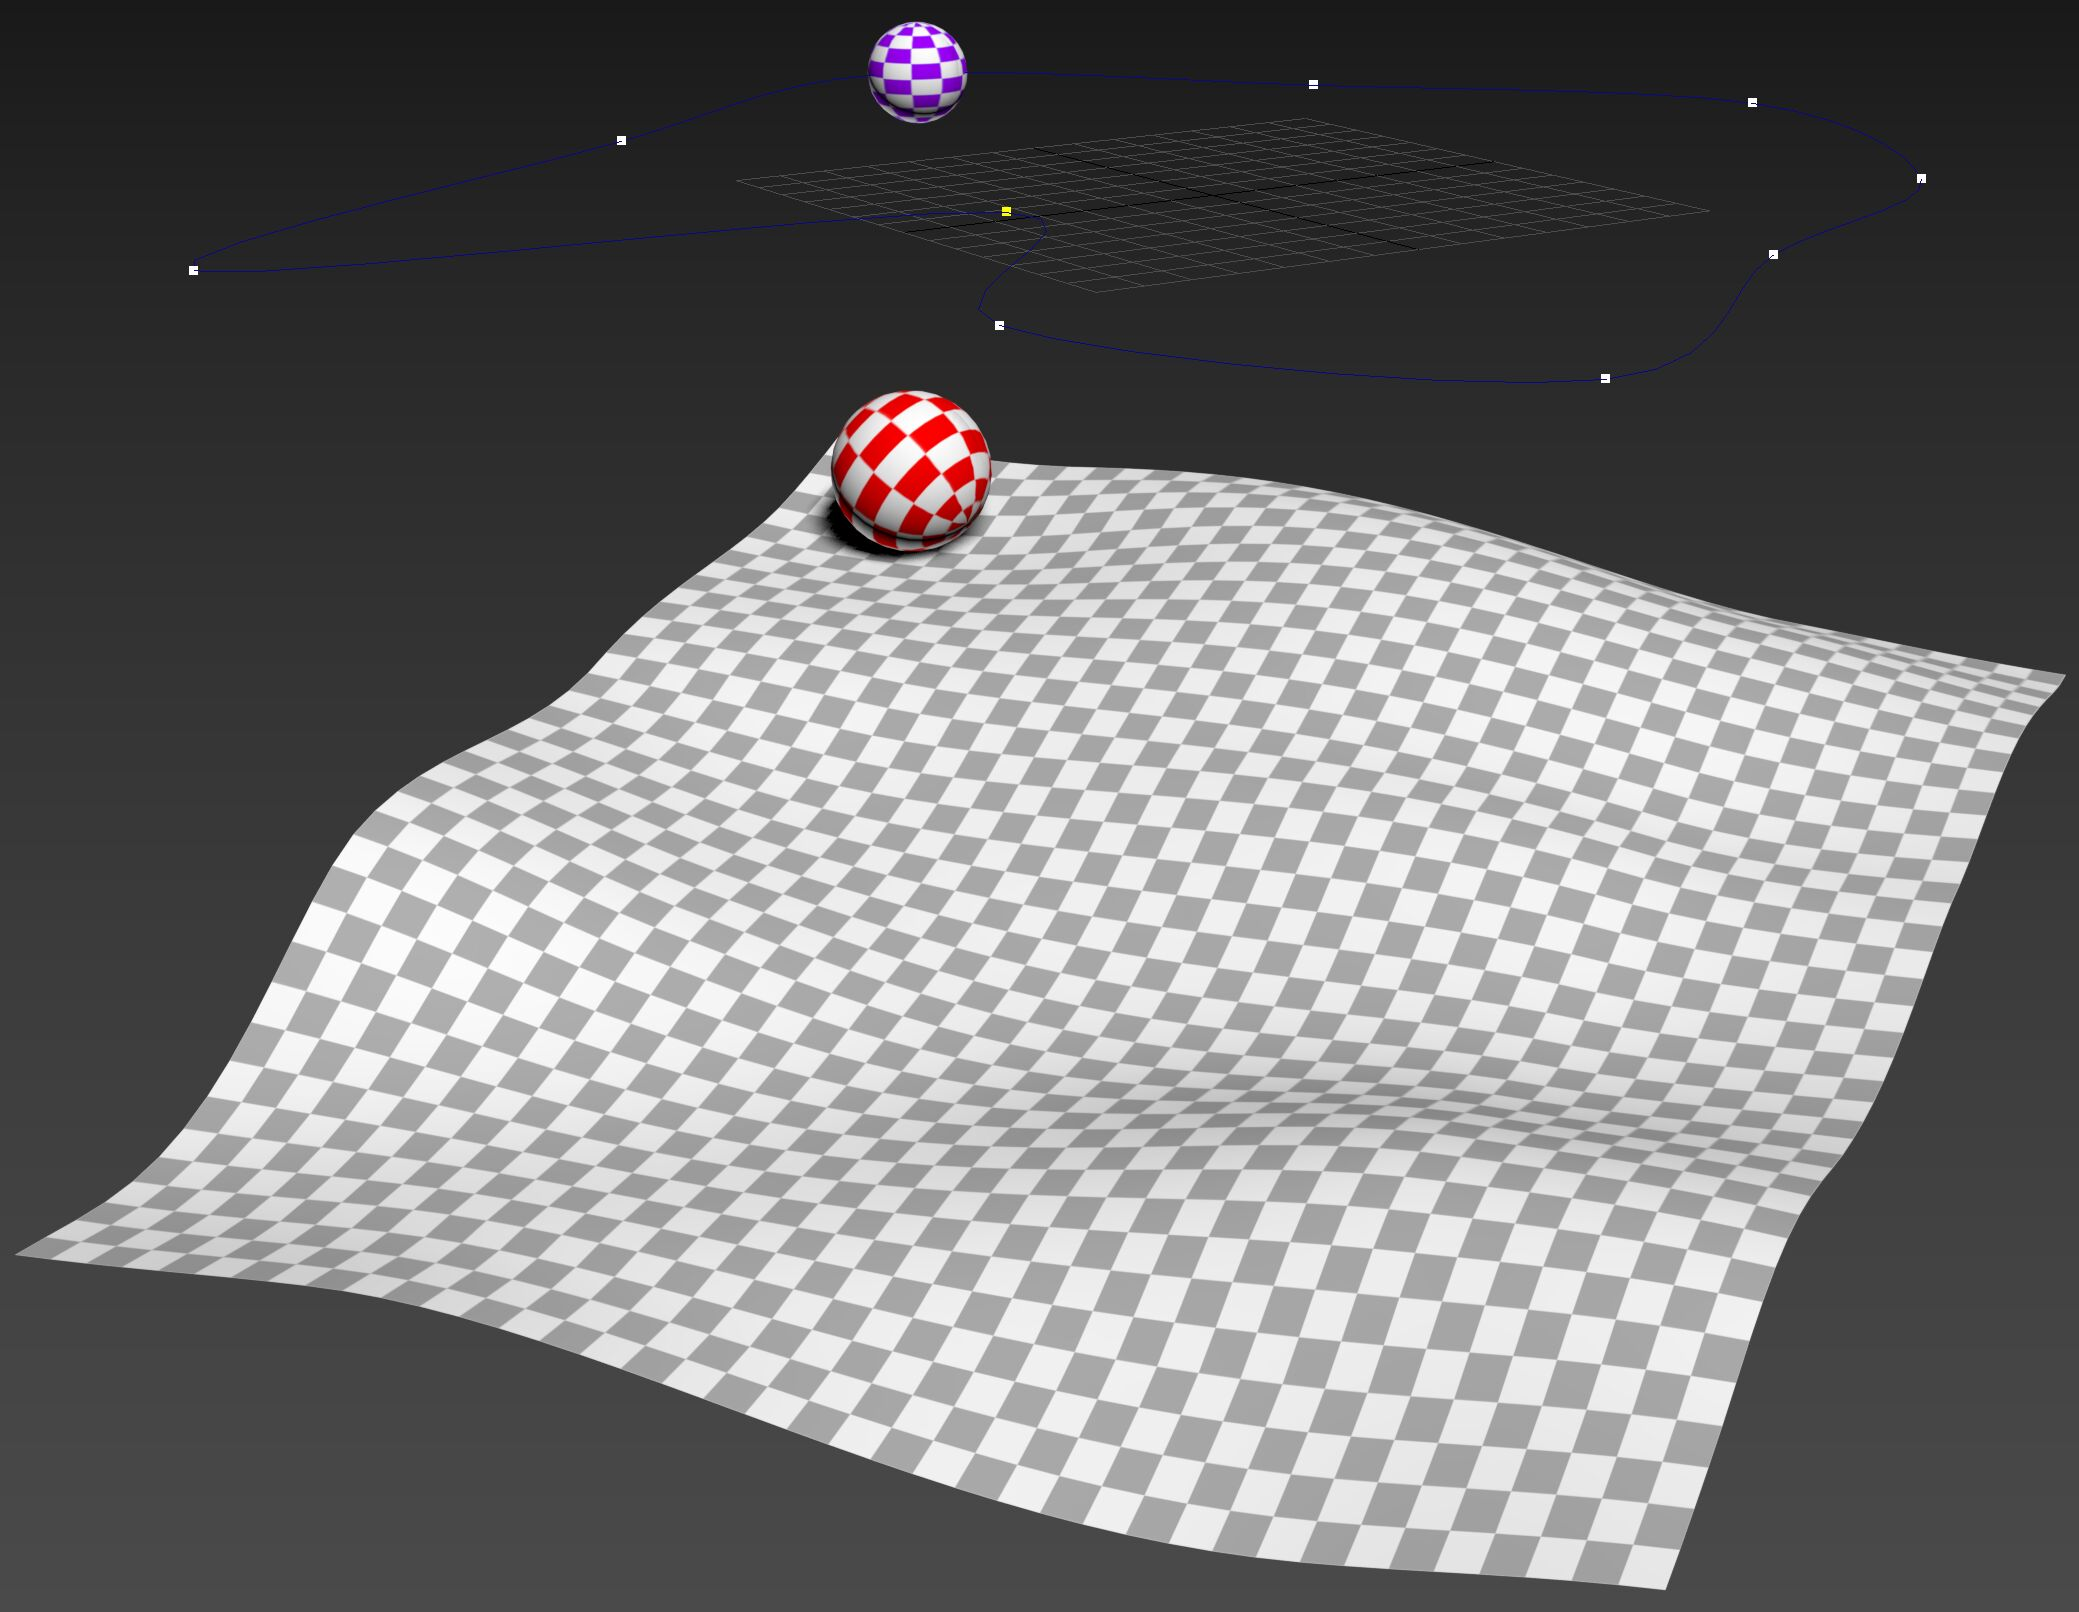
\includegraphics[width=\textwidth]{imagenes/rotacion/185.jpg}
        \caption{Pelotas en el instante 185.}
    \end{subfigure}    
    \par\bigskip
	\begin{subfigure}[t]{0.48\textwidth}
	    \centering
	    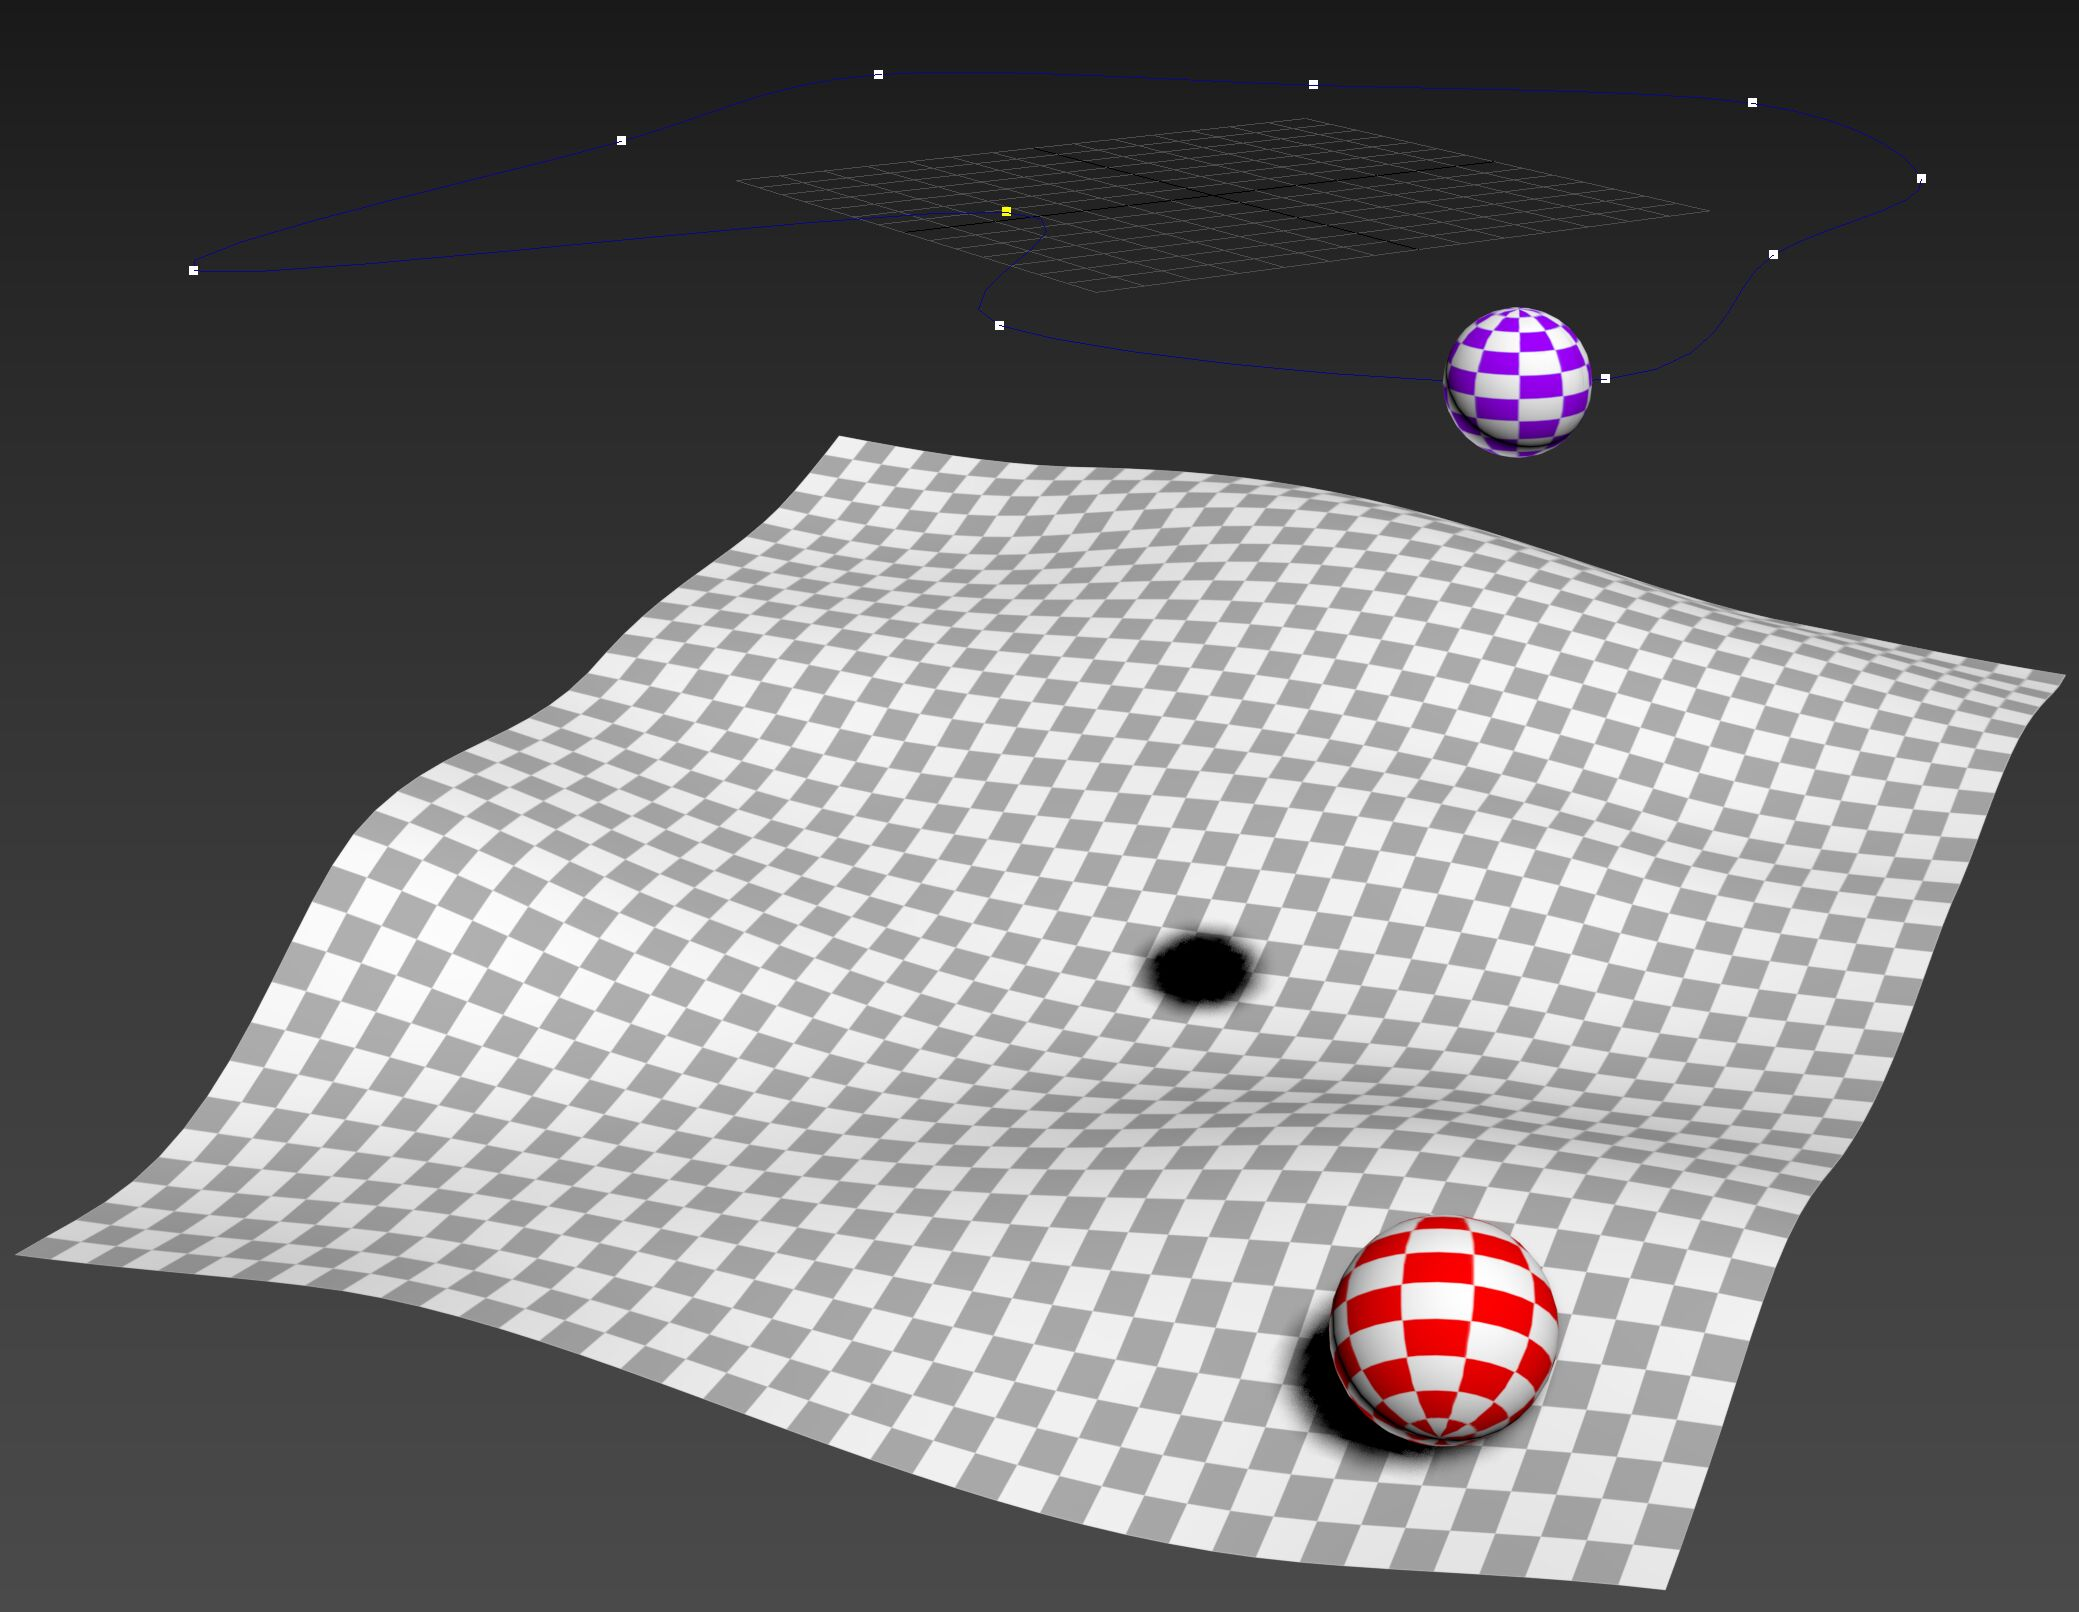
\includegraphics[width=\textwidth]{imagenes/rotacion/410.jpg}
        \caption{Pelotas en el instante 410.}
    \end{subfigure}        
    \caption{Visualización de algunos instantes de la animación final.}
\end{figure}

% \bibliographystyle{plainurl} % We choose the "plain" reference style
% \bibliography{bib} % Entries are in the refs.bib file

\end{document}
